
\section{Models validation}
\subsection{IC substrate thinning}
As substrate thinning is quite widespread when performing fault injection, let us have a quick look on how it is performed.
Commonly, It is done using Selected Area Preparation (SAP) machines.
They consist in very precise milling tools, generally able to remove material with a precision down to a few micrometers.
In addition to substrate thinning, these machines allow removing the plastic package and eventual internal metallic heat-sinks of ICs.
It has the advantage of providing low damage to thinned ICs, thanks to low spindle speed and low temperature rise compared to traditional high speed milling.
Additionally, it is possible to polish the thinned surface in order to have a smooth physical environment to work with BBI probes.

\subsection{Substrate thinning experiments}
\begin{figure}[ht]
    \centering
    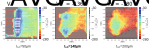
\includegraphics[width=\textwidth]{4_thinning/figures/cartosFautesNew.pdf}
    \caption{Fault susceptibility maps}
    \label{fig:fsm1}
\end{figure}
\begin{figure}[H]
    \centering
    \includegraphics[width=16cm]{4_thinning/figures/cartosFautesSpreading.png}
    \caption{Susceptibility area spreading}
    \label{fig:fsm1spread}
\end{figure}
\begin{figure}[H]
    \centering
    \includegraphics[width=16cm]{4_thinning/figures/cartosCouples.pdf}
    \caption{Fault susceptibility maps couples}
    \label{fig:fsm1couple}
\end{figure}
With geometric and electrical modeling complete, it is now possible to conduct experiments in order to verify the meaningfulness of the previous approach.
For this purpose, three experiments were performed and are described in the next paragraph.

The first one aimed at measuring the minimal voltage pulse amplitude $V_{PU}^{MIN}$ required to induce a fault on an IC performing computations.
The obtained results are called fault susceptibility maps (FSM).
They allow spotting the region where the IC is sensitive to BBI, no matter which type of induced fault.
Fig. \ref{fig:fsm1} presents three traditional fault susceptibility maps for three identical ICs, with different substrate thicknesses.
From left to right, $t_{SUB}$ goes from 50 µm, then to 140 µm, finally to 200 µm.
In each case, the maps are performed above the hardware AES core of the IC, temporally aiming the penultimate AES round.
The scanned area measures 1.7 mm by 1.7 mm.
$V_{PU}$ was limited to the following range: [30 V ; 280 V], with 5 V steps and a negative polarity.
The pulse width was fixed at 6 ns.
